\chapter{Literature review}\label{cha:litterature}

This chapter is literature review of potential novelty detection techniques and methods for feature extraction and dimensionality reduction. 

% \section{Novelty vs anomaly(outlier) detection}
%     \cite{Pimentel2014} explains that an outlier or anomaly is a data point that is inconsistent with the rest of the dataset, but it is also used as a term to describe normal data that is far from the normal data point. This means that an outlier is not necesarily an unwanted data point, just an extreme. Outliers have a big impact when construction models, and if a data point is an outlier it is either very important to include or critical to exclude.
    
%     Clarify the two expressions, what is the difference between them? what is not? 
%      "Two interchangeable synonyms of novelty detection
%         [21,1] often used in the literature are anomaly detection and outlier detection [22]. The different terms originate from different domains of application to which one-class classi- fication can be applied, and there is no universally accepted definition.Merriam-Webster [23] defines “novelty” tomean “new and not resembling something formerly known or used”. Anomalies and outliers are two terms used most commonly in the context of anomaly detection; sometimes interchangeably [24].Barnett andLewis [25] define an outlier as a data point that “appears to be inconsistent with the remainder of that set of [training] data”. However, it is also used to describe a small fraction of “normal” data which lie far way from the majority of “normal” data in the feature space [9]. Therefore, outlier detection aims to handle these “rogue” observations in a set of data, which can have a large effect on the analysis of the data. In other words, outliers are assumed to contaminate the dataset under consideration and the goal is to cope with their presence during the model-construction stage." quote from \cite{Pimentel2014}
\section{Novelty detection}\label{sec:novelty_detection}
    \cite{Pimentel2014} defines novelty detection as the task of classifying test data that in some way differs from data used for training. This is like a one sided test or one class classification. This means that one is not training on data that represents fault, only on data sampled from normal operation. As a model describing the normal operation of the system is learnt, it is important that one have samples of normal system behaviour for all the possible states of operation. Novelty detection avoid the issue with finding data that represents all possible failure modes. Such techniques are very valuable for industry applications, where the need for failure detection is great, but identifying all possible failure modes and collecting data to represent it can be difficult and very costly. It is much easier to get measurements from a machine during normal operation, than during failure. This means that it is close to impossible to obtain as many samples of negative or faulty data as of normal data. \cite{Tarassenko2009} claims that modern high-integrity systems are so complex that they introduce many possible failure modes that are not very well captured by the instrumentation available. This can be verified by visiting a hydro electric power plant. There is a lot of instrumentation, and many alarms for different components, but all of these are linked to well known failures. Novelty detection introduces the possibility to detect unknown abnormalities. 
    
    Since novelty detection is trained on "normal" operation data, it should be able to detect any abnormal situation that can occur. By adding more process signals to the system than what is used in the normal failure detection system, one can enable the novelty detection system to detect new failure states. This leads to an important remark, only getting a notification that a novelty is observed, does not provide very much information. For these techniques to have any real value, one need to be able to trace which component the novelty comes from. Once the novelty detection technique is trained, new data are given a novelty score based on how well they compare to the normal description of the system. This score can then be compared to a threshold, and the data will be marked as normal or abnormal.

    Many of the techniques in the following sections are based on the suggestions from \cite{Pimentel2014} which provides an extensive review of novelty detection. 

\section{Reducing the number of features}\label{sec:reduce_features}
    
    There are two main techniques for reducing the feature size, feature selection, and dimensional reduction. The former, tries to remove the least informative and the redundant features from the feature set. The latter creates new features either as linear or non-linear combinations of the original feature set, hence one can remove the dimensions which brings little data variance to the table. Feature selection is again separated into supervised and non-supervised selection. In the supervised case, one have a set of features and a target variable, hence one want to keep the features that is related to the target variable. For unsupervised feature selection, there is no target variable to help remove uninformative or redundant features, there is no way to confirm that the best subset of features are selected, and this area is not researched as much as the supervised case. \cite{Liu2010} states that some features can be removed without lowering the performance of a learning algorithm. 
    
    
\section{Feature selection}\label{sec:feature_selec}
    The dataset presented in chapter \ref{cha:data} is a large dataset, it contains data from a period of four years, and holds a total of $251$ process variables or features. Analyzing a dataset with $251$ features is not a trival task. Interpreting and visualizing data of such high dimensions is almost impossible. The feature size also introduces issues regarding memory and algorithm runtime, \cite{Guyon2003} and \cite{Dy2004}. Reducing the complexity of the problem is heavily correlated with reducing the number of features. Feature selection techniques can also reveal unknown plant dynamics which can help to understand why some components fail.
    
    "The problem is that not all features are important. Some of the features may be redundant, some may be irrelevant, and some can even misguide clustering results" from \cite{Dy2004} sums up one of the issues with datasets with many features. A concrete example of this is shown in figure \ref{fig:feature_selection}, her one can clearly see that $X_2$ does not provide any information on how the datapoints are clustered. Including this feature in a learning algorithm does not provide any information about the two classes of data found in the dataset, hence in best case the performance will be the same as if only $X_1$ was used.  
    
    \begin{figure}
        \centering
        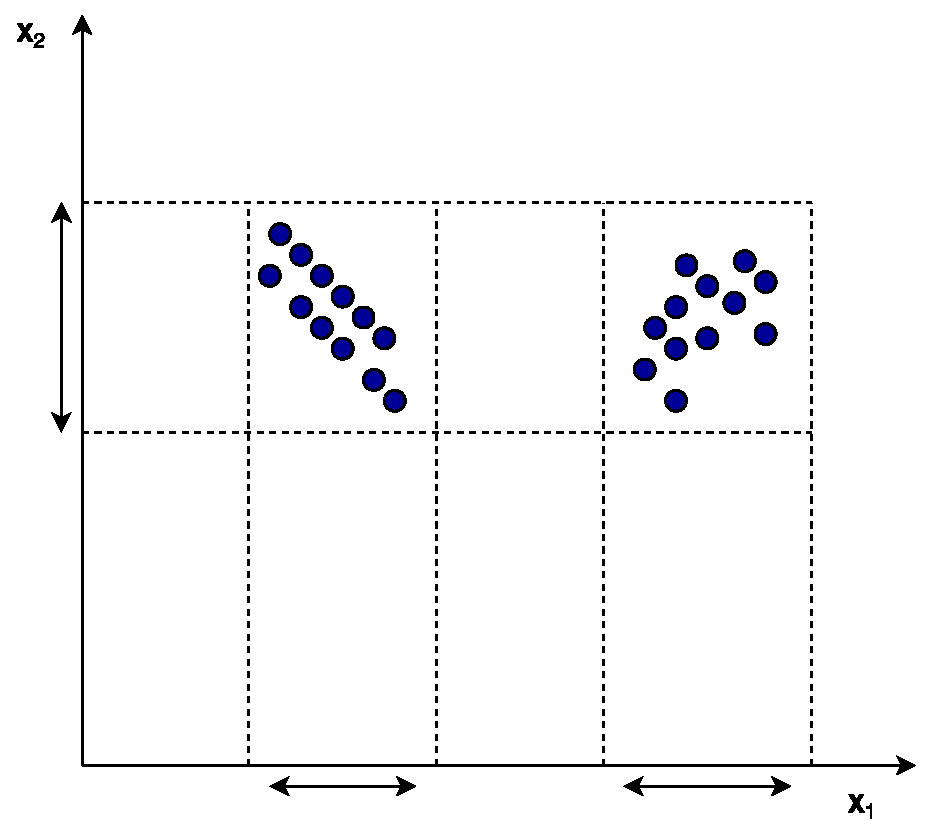
\includegraphics[width=0.5\textwidth]{report/figures/techniques/feature_selection.pdf}
        \caption{Example of a two-dimensional dataset, with one relevant and one irrelevant feature}
        \label{fig:feature_selection}
    \end{figure}
    
    
    
    \subsection{Filter, wrapper and embedded methods}\label{subsec:filter_wrapper_embedded}
    The different classes or types of methods for feature reduction are split into three groups. This section will give a short introduction to each of them.
    According to \cite{Liu2010} filter methods are methods that perform feature selection separate from the learning algorithm, and hence can be used no matter which learning algorithm is applied later. The wrapper methods however, need a predetermined learning algorithm. The features are then selected based upon the performance of the chosen algorithm.  Finally the embedded methods incorporate the selection of features in the training of the learning algorithms model.
    \cite{Liu2010} also states that since the filter methods are independent from the learning algorithm they are not biased with regard of the algorithm. Since different feature sets selected by different methods are to be tested on the same learning algorithms, this is seen as beneficial, and hence only filter methods are used in this thesis. 

\section{Supervised feature selection}\label{sec:sup_feat_select}
    Supervised feature selection can be used when you have a target to track. This means that you need to identify a process signal or a function of a process signal of interest which you want to trace in the other process variables. An example is novelty detection for a bearing. By using process variables from the bearing such as vibration and temperature, one can find other process variable that are in some way related to the targets. 
    % As seen in chapter \ref{cha:data} the control problems with the needles can be observed in the difference or the RMSE between the pairwise controlled needles. Using the RMSE between the needles as a target variable enables the use of supervised feature selection algorithms. 
    
    
    \subsection{K-best using correlation and  mutual information}\label{subsec:K-best_feat_select}
    
        Mutual information, \cite{Kraskov2004} and \cite{Peng2005} explains how dependent or inversely how independent two variables are. It gives an understanding on how much knowing something about one variable reduces the uncertainty about the other. If two variables are completely independent, their corresponding mutual information or MI will be zero. 
        
        The mutual information is defined as
        \begin{align}\label{eq:tech_MI}
                MI(X,Y) = \int \int p(x,y) \log \frac{p(x,y}{p_x(x),p_y(y)},
        \end{align}
        where $x$ and $y$ are the two variables to compare, and $p(x)$ and $py(y)$ is their corresponding probability density functions. One benefit from MI is that does not only find linear correlation between two variables. In other words, it finds dependencies between variables not necessarily shown in correlation, meaning that this serves as complementary technique to using co-variance or correlation for feature selection, \cite{Li}. The K features with highest MI will be chosen. 
        
        
        The K-best features can also be selected using the above mentioned correlation. The correlation between a feature and the target variable is found as  
        \begin{align}
            corr(X,Y) = \frac{cov(X,Y}{\sigma_x\sigma_y} = \frac{E[(X-\mu_x)(Y-\mu_y)]}{\sigma_x\sigma_y}.
        \end{align}
        Here the K features with highest correlation with the target variable will be chosen. 
        
\section{Unsupervised feature selection}\label{sec:unsup_feat_reduc}
    Unsupervised feature selection is harder than supervised feature selection. The lack of a target variable, removes the ability to easily interpret which variable dynamics that are important. Still the need to reduce the feature set is prominent. \cite{Dy2004} describes the problem as follows, "The goal of feature selection for unsupervised learning is to find the smallest feature subset that best uncovers “interesting natural” groupings (clusters) from data according to the chosen criterion". The chosen criterion defines what is thought to be interesting natural groupings. As they go on to explain, there is no one optimal golden rule for defining this criterion, and a subset that is good for one purpose might not be relevant for others. The two methods chosen for unsupervised feature selection follows. \cite{He2005} states that feature selection based on data variance is one of the simplest evaluation methods, and hence it is a natural element of the analysis. 
    
    
    \subsection{Variance threshold}\label{subsec:var_thres}
    
        One of the drawbacks with using variance to select features, is that there might be a lot of features with large variances that is non-informative with what one is looking for. The algorithm is very simple, it returns the k features that has the highest variance. 
        
    
    \subsection{Laplacian score}\label{subsec:lapl_score}
        Laplacian score for feature selection was proposed as an alternative to unsupervised feature selection by \cite{He2005}. The method builds upon the assumption that features belonging to the same class or grouping will be close. The features are evaluated based on how well locality is preserved, which is found by the Laplacian score. The Laplacian score is calculated for each feature. A short introduction to the method is described below, more details can be found in \cite{He2005}. 
        
        Laplacian score is based on Laplacian Eigenmaps \cite{laplcian score for feature selection}, which is an algorithm for dimensionality reduction. The algorithm creates a nearest neighbors graph with a node for each sample of each feature. Hence the dimension becomes $m$x$\#features$. Two nodes share an edge if they are among the k-nearest neighbors to each other, meaning that k is one of they tunable parameters for this algorithm. Each edge is then given a weight based on the Gaussian radial basis function;
        
        \begin{align}\label{eq:tech_LS}
            W_{i,j} = e^-{\frac{||{\bm{X_i}-\bm{X_j}}^2||}{t}},
        \end{align}
        
        where t is another tunable parameter. Then a graph Laplacian is computed which then again is used to calculate a Laplacian score. As mentioned the algorithm has two tunable parameters. The main reson for choosing Laplacian score as one of the unsupervised feature selection methods, is that it has the ability to compare and rate features against each other. This introduces a new dimension compared to the more naive variance threshold algorithm, that only looks at one feature at a time. 
    

\section{Dimensionality reduction}\label{sec:dim_red}
    One of the issues with feature reduction is that the features that are removed, may hold information that could help the learning algorithm. In dimensional reduction, the feature set is used to create new features which means that a new reduced feature space of dimension n can hold the same amount of information as the original feature space of size m, $m>n$.

    \subsection{PCA}\label{subsec:PCA}
        Principal component analysis, is one popular technique used for dimensional reduction. PCA is an orthogonal transformation that takes a set of possibly correlated variables, and transforms them into a set of non correlated components, effectivly reducing the dimensions of the data. These new dimensions are known as principal components. There are several different algorithms that can be used to calculate the principal components, one of them is singular value decomposition or SVD. SVD decomposed the data into eigenvalues and eigenvectors. The larger a eigenvalue is, the better its corresponding eigenvector capture the variance of the data. All eigenvectors are orthogonal, this means that each vector introduces an entirely new dimension. In a high dimensional dataset with many features, there will most likely be features that are fairly similar. Figure \ref{fig:tech:PCA} shows intuitively how the PCA algorithm works. Data samples from a dataset with three features are shown in the plot. As the principal components in red and green shows, most of the variance in the samples can be represented using only one dimension. Adding the second dimension, only small residuals might be left. This illustrates how the PCA algorighm operates. 
        
        \begin{figure}
            \centering
            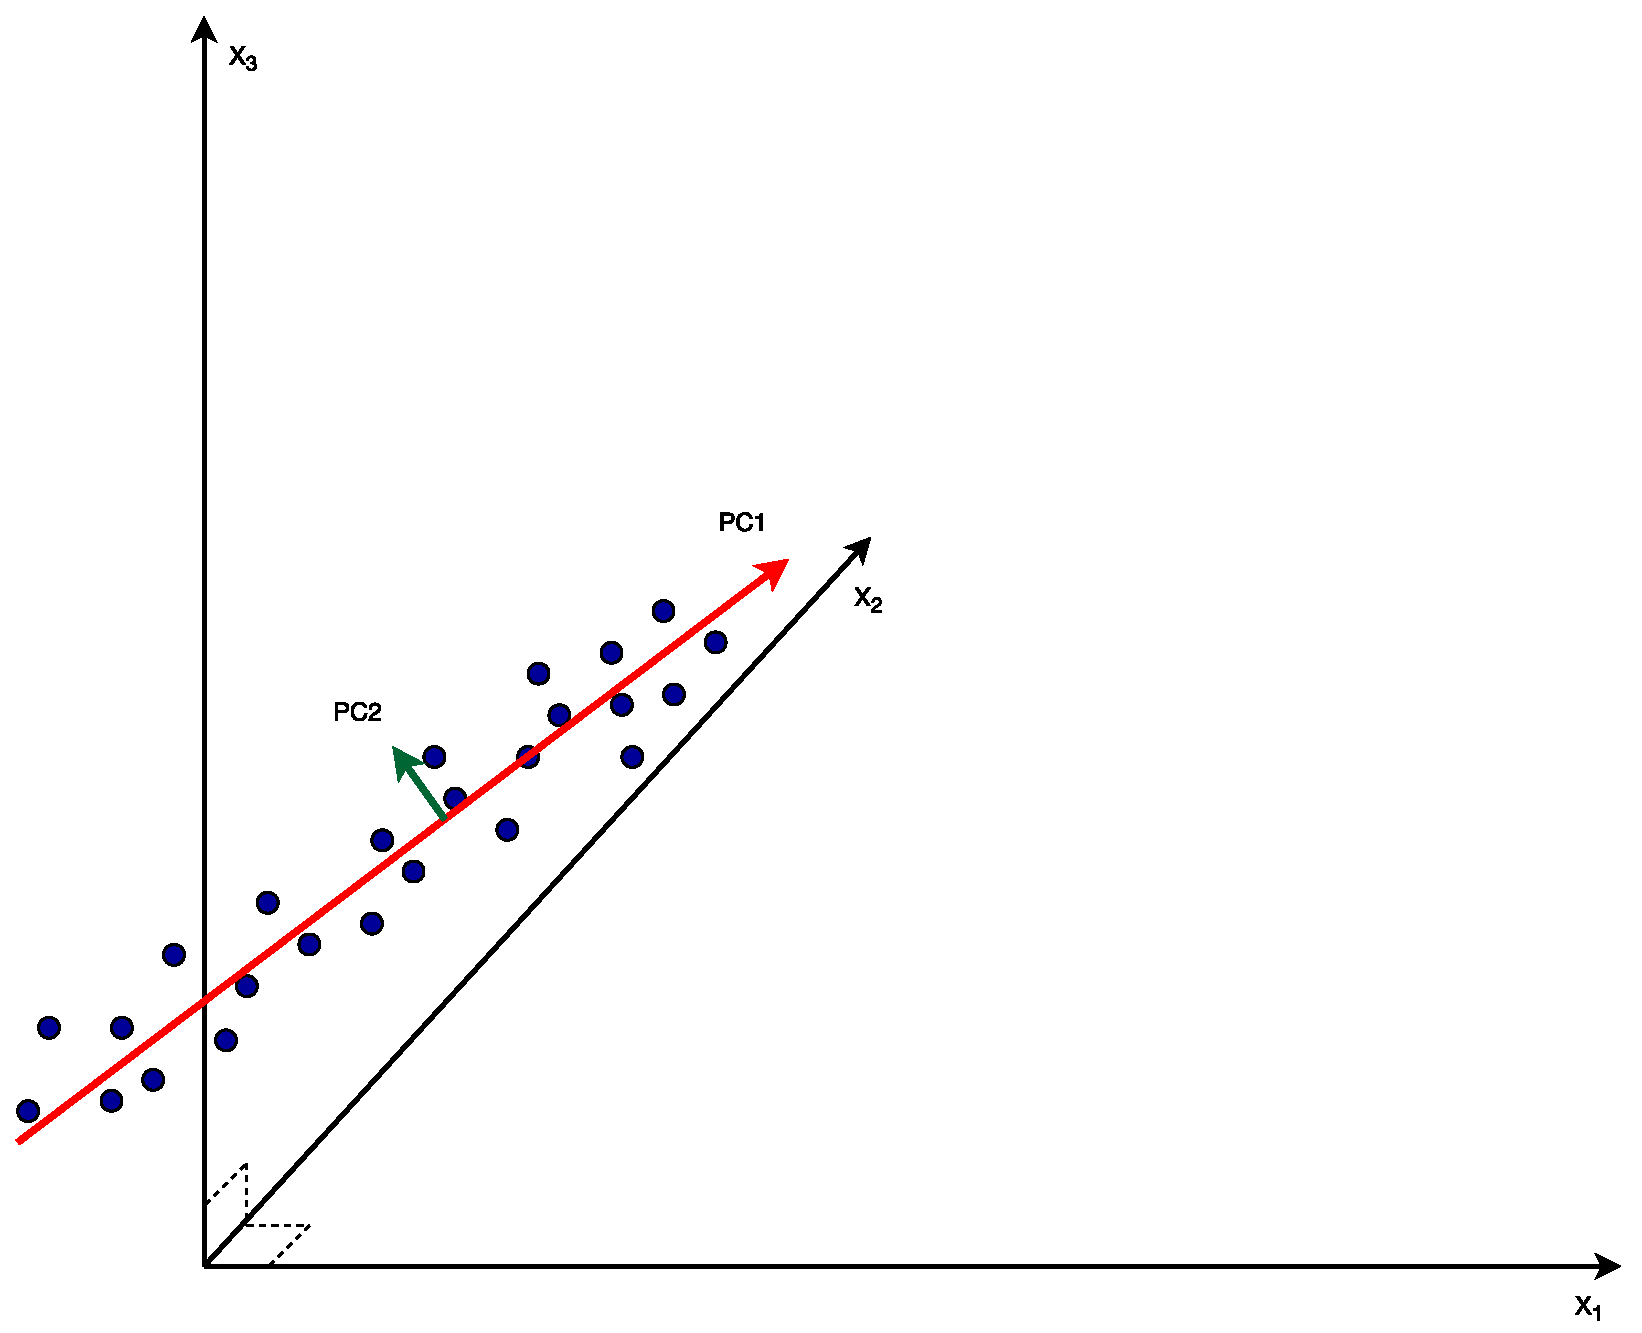
\includegraphics[width=\textwidth]{report/figures/techniques/PCA.pdf}
            \caption{Illustration on how principal component analysis work}
            \label{fig:tech:PCA}
        \end{figure}
        
    
    \subsection{Kernel PCA}\label{subsec:kernelPCA}
        Kernel PCA builds upon the PCA algorithm explained above, but it introduces a new trick. Where PCA is only able to create new features from linear combinations of the original feature set, kernel PCA uses the kernel trick to enable non-linear combinations as well. Say you have a two dimensional dataset containing samples from two different classes.  These classes are only linearly separable if the classes can be separated by a line. If one class surrounds the other class, there is no way to linearly separte the two clases in two dimensions. However, by extending the sample space into three dimensions, it might now be possible to separte the two classes with a hyperplane. Hence making a non-linear separation of the two classes possible, by still using linear methods. If the datasets are large, transforming all samples into a higher dimension can become computationally heavy. The kernel trick solves this problem without having to transform the samples. The kernel PCA extends the original PCA to a higher dimension using the kernel trick, enabling the extraction of nonlinear components.  
    
        By mapping the original data nonlinearly into a new feature space $F$ $\phi(\bm{x_1})$, and by performing PCA in this new feature space, one can get nonlinear principal components.

\section{Anomaly detection}\label{sec:Anomaly_detection}
    
    \subsection{One class SVM}\label{subsec:OCSVM}
    
            The following section is a summary based on my project thesis written the fall of 2017.
            
            Support vector machine or SVM, can be used for both supervised and unsupervised learning. In the unsupervised case, it is most commonly used for outlier and boundary detection. For supervised learning it handles two classes at a time, so one vs the rest is used if there are more than two classes. The classifier defines a hyperplane that separates the two different classes. The hyperplane can then later be used to predict which class a new feature vector belongs to.  
            
            SVM is capable of separating data both linearly and nonlinearly. How the algorithm separates the data depends on the kernel function it uses. A kernel function, or a similarity function, describes how similar two feature vectors are by taking the inner product of the two samples in a higher dimensional space. The kernel function does this without having to explicitly transform the data into this dimension.
            
            Two commonly used kernels are the Gaussian kernel
            \begin{align}
                K_g(\bm x^{1},\bm x^{2}) = e^{\frac{\norm{\bm x^{1}-\bm x^{2}}^2}{2\sigma^2}}, 
                \label{svm:gauss}
            \end{align}
            and the polynomial kernel
            \begin{align}
                K_p(\bm x^{1},\bm x^{2}) = (\bm x^{1T}\bm x^{2} + \alpha)^\beta.
                \label{svm:poly}
            \end{align}
            
            is another example of a kernel function. These are just two of many examples. The Gaussian or RBF kernell is a good first choice if you know that you have a nonlinear boundary, but don't know exactly what shape the boundary will take. If you have more knowledge about the shape of the boundary you are looking for, you might want to consider more special kernels.
    
            
            One of the great benefits of the SVM algorithm is that the solution is found by Lagrangian optimization problem 
             \begin{align}
                L = \sum_{i=1}^n  \alpha_i - \frac{1}{2} \sum_{i=1}^n \sum_{j=1}^n \alpha_i \alpha_j y^i y^j \bm x^{iT} \bm x^j,
                \label{svm:dual}
            \end{align}
            which is a convex optimization problem, and hence it has a global maxima.
            
            
            If your classes are not linearly separable in the feature space, maximization of Equation \ref{svm:dual} has no global solution. However as can be seen in Equation \ref{svm:dual} one want to minimize $\bm x_i^T  \bm x_j$. This term can then be replaced by one of the kernel functions defined above, which now enables separation in a higher dimensional space.
            
            The final thing to remark is that not all datasets are completely separable, to deal with this a slack variable is introduced into the optimization to allow miss-classification of some of the feature vectors. 
        
    
        One issue with one class svm combined with non labeled data, is that hyperparameterization becomes hard. There is no out of the box scoring function that tell you how well the classifier is performing. As long as one is working in two or three dimensions it is possible to plot the decision boundary, and select parameterization based on visual observations. In higher dimensions this becomes a proble, therefor a new method is proposed used to reduce the number of hyperparameterizations to consider. A score is given each of the paramterization from
        
        \begin{align}
            score = \abs\sigma + \mu + 100\frac{outliers}{inliers},
        \end{align}
        where the lower the score, the better the performance. $\sigma$ here represents the standard deviation of the distances from the decision boundary, $\mu$ is the unsigned distance to the decision boundary. These values were picked because the training data is said to be normal operation, and should not contain any outliers. However, this leads to the risk of a to general boundary where the classifier is no longer able to predict outliers. This means that the closer the boundary is to the samples in the training data, the higher the score. The final fraction of outliers and inliers is added to make sure that most of the data is classified as inliers. If not on runs the risk of fitting av very complex boundary which yields good distance measures for all samples, this will however lead to a large fraction of outliers which is not the case for the normal training data. 
        
        
    
    \subsection{Kernel density estimation}\label{subsec:kde}
        Kernel density estimation creates and estimate to the probability density function or pdf of the data. This is a non-parametric technique meaning that the data is not assumed to take the shape of a given distribution. The probability density function is estimated using a set of kernels that are distributed across the data. The probability density is then estimated at each kernel location based on data that lie within a local neighborhood of the kernel. The density found at a point x within its neighboring n points is given by, 
        \begin{align}
            \hat{f}(x) = \frac{1}{n} \sum_{i=1}^n K_h(x-x_i)  = \frac{1}{nh} \sum_{i=1}^n K(\frac{x-x_i}{h}).
        \end{align}
        Here the $K()$ is the kernel function, and $h$ is a tunable hyperparameter for variance known as the bandwidth. This parameter smooths the distribution. The kernel function can take on a number of forms, where the gaussian kernel,
        \begin{align}
            K(x-x_i;h) = e^-\frac{||x-x_i||^2}{2h^2}
        \end{align}
        is the most commonly used. 
        
        
    % \subsection{K-nearest neigbours}\label{subsec:k_neig}
    %     outliers are datapoints that are far from the normal observations. 
        
    % \subsection{Timeseries forecasting using Neural Networks}\label{subsec:NN}
    %     present even if it will not be used due to the lack of consistency in the timeseries 
    %     Finne ein paper og citere på normal timeseries forecastin, denne vil eg då ikkje bruke sidan eg har aperiodisk sampling! 
    \subsection{Timeseries forecasting}
    
    
    \subsection{LSTM}
    
    Long Short Term Memory Networks or LSTM is a type of neural network, and is proposed as a scheme for anomaly detection in \cite{Malhotra2016} and \cite{Malhotra}. It is shown that the scheme is working for both periodic and aperiodic timeseries. 
    A LSTM network is a reccurent neural network, that have been successfully used for handwritten text recognition and speech recognition. The paper proposes a an encoder-decoder scheme designed for anomaly detection. A timeseries is encoded, and then decoded back to reconstruct the input series. The reconstruction error, the error between the input and the reconstructed input is then used to identify outliers. In the training phase the system is only shown normal data, hence it only learns to reconstruct the normal system behaviour. The network should then not be able to reconstruct anomalous data as good as with normal data. The paper concludes that LSTM networks can be a viable approach for anomaly detection. It also shows promise in detecting anomalies from unpredictable time-series.      
    
